%\documentclass{beamer}
%\documentclass[notes=only]{beamer}   % only notes
\documentclass{beamer}              % only frames

\usetheme{simple}

\usepackage{lmodern}
\usepackage[scale=2]{ccicons}
\usepackage[T2A]{fontenc}
\usepackage[utf8]{inputenc}  
\usepackage[russian]{babel}
\usepackage{listings}
\usepackage{geometry}
\usepackage{marginnote}
\usepackage{movie15}
  
% TODO: 
%   position adjustement
%   change colours
%       

% Watermark background (simple theme)

%\setwatermark[hoffset=2cm,voffset=1,5cm]{
\includegraphics[height=8cm]{img/watermark1.png}}
\setwatermark{
\includegraphics[height=9cm]{img/watermark1.png}}


\title{О некоторых преобразованиях для высокоуровневого синтеза на ПЛИС}
\subtitle{}
\date{\today}
\author{Баглий Антон}
\institute{\url{sfedu.ru}}

\begin{document}

\maketitle


\begin{frame}{ПЛИС}
  \framesubtitle{Что это такое}
   
  \begin{columns}
    \column{.7\textwidth}
      \begin{itemize}
        \item микрочип из большого набора однотипных элементов, связи между которыми можно настраивать
        \item набор ПО от производителя для компиляции низкоуровневого описания схемы под конкретный чип
        \item удобная платформа для любой вычислительной электроники
      \end{itemize}

    \column{.3\textwidth}
      \begin{block}{В целом}
         Возможность сконструировать любую электронную схему
      \end{block}
  \end{columns}		  
\end{frame}

\begin{frame}[fragile]
\frametitle{ПЛИС}
  \framesubtitle{Как они программируются}
  \begin{columns}
    \column{.2\textwidth}
      \begin{itemize}
        \item VHDL
        \item Verilog
      \end{itemize}
      
      \begin{block}{Низкий уровень}
         Тяжелее в написании и отладке. 
      \end{block}

    \column{.8\textwidth}
      
      
\begin{lstlisting}[frame=single]
begin
  regs : process (clk, rstx)
  begin  -- process regs
    if rstx = '0' then         
      r1reg <= (others => '0');
    elsif clk'event and clk = '1' then  
      if glock = '0' then
        if t1load = '1' then
          case t1opcode is
            when OPC_CALCINDEX32 =>
              r1reg <= (others => '0');
              r1reg <= (t1data + 1) mod 4 + t2data * 4;
            when others =>
              null;
          end case;
        end if;
      end if;
    end if;
  end process regs;
  r1data <= r1reg;
end rtl;
\end{lstlisting}
\label{clone_listing}
      
  \end{columns}
  
\end{frame}

\begin{frame}[fragile]
\frametitle{ПЛИС}
  \framesubtitle{Как они программируются}
  \begin{columns}
    \column{.2\textwidth}
      
      По этой программе придется создать набор взаимодействующих конечных автоматов,
         читающих и записывающих данные.

    \column{.8\textwidth}
      
      
\begin{lstlisting}[frame=single]
for (i = 0; i < length - k; i++)
bb[i] = 0;
 for (i = k - 1; i >= 0; i--) {
  feedback = data[i] ^ bb[length - k - 1];
   if (feedback != 0) {
    for (j = length - k - 1; j > 0; j--)
	 if (g[j] != 0)
	  bb[j] = bb[j - 1] ^ feedback;
	 else
	  bb[j] = bb[j - 1];
	  bb[0] = g[0] && feedback;
	 } else {
	  for (j = length - k - 1; j > 0; j--)
	   bb[j] = bb[j - 1];
	   bb[0] = 0;
	  }
}
\end{lstlisting}
\label{encode_listing}
      
  \end{columns}
  
\end{frame}

% turn off watermark
\setwatermark{}

\begin{frame}{Высокоуровневый синтез}
  \framesubtitle{Как построить конвейер}
  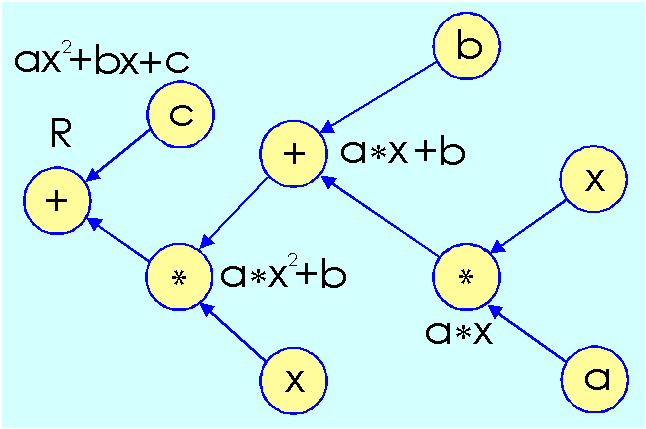
\includegraphics[height=8cm]{img/CalcGraphExample.png}
\end{frame}

\begin{frame}{Высокоуровневый синтез}
  \framesubtitle{Сложности}
  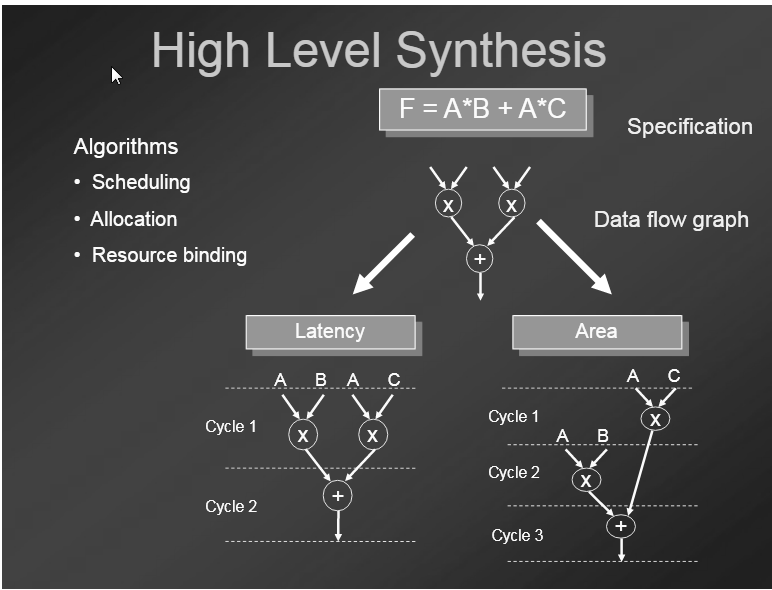
\includegraphics[height=9cm]{img/HLSFlow1.png}
\end{frame}

\begin{frame}{Архитектуры}
  \framesubtitle{Что такое IP-ядро}
  
  \begin{columns}
    \column{.5\textwidth}
      \begin{itemize}
          \item MicroBlaze
          \item Nios II
          \item MIPS
          \item ... и сотня других
  		\end{itemize}

    \column{.5\textwidth}
      \begin{block}{Зачем это}
         Можно не преобразовывать всю программу целиком в электронную схему,
         а добавить в готовый универсальный процессор свои расширения (сопроцессор, новые инструкции).
      \end{block}
  \end{columns}	
  
  
\end{frame}

\begin{frame}{Архитектуры}
  \framesubtitle{VLIW и параллелизм инструкций}
  \begin{itemize}
          \item Несколько операций одной командой
          \item Набор функциональных модулей
          \item Регистровый файл как узкое место
  	\end{itemize}
  
\end{frame}

\begin{frame}{Архитектуры}
  \framesubtitle{TTA-архитектуры}
   \begin{itemize}
          \item Простота модицикации
          \item Более сложный компилятор
          \item Проще экспериментировать с диапазоном характеристик разрабатываемой схемы
  	\end{itemize}
  \nocite{Corporaal1994}
\end{frame}

%\begin{frame}{Архитектуры}
%  \framesubtitle{Простота модификации}
%  
%\end{frame}

\begin{frame}{Архитектуры}
  \framesubtitle{Сo-design}
  
\end{frame}

\begin{frame}{Code factoring}
  \framesubtitle{GCC, SSA}
  \nocite{Loki2004}
  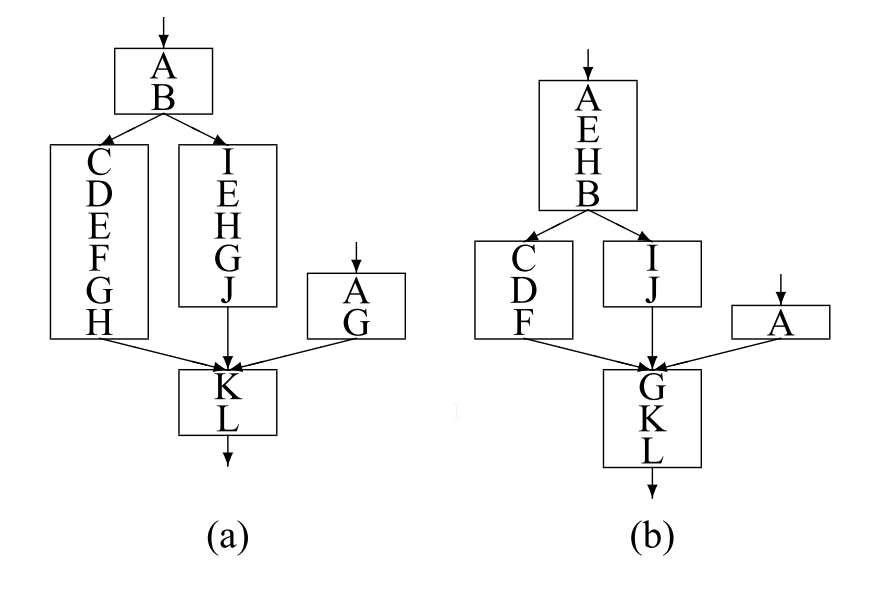
\includegraphics[height=8cm]{img/CodeFactoring.png}
\end{frame}

%\begin{frame}{Code factoring}
%  \framesubtitle{Outlining}
  \nocite{Zhao2005}
% 
%\end{frame}

%\begin{frame}{Code factoring}
%  \framesubtitle{клоны в исходном коде}
%\end{frame}

\begin{frame}{Клоны}
  \framesubtitle{Алгоритмы поиска}
   \begin{itemize}
          \item Поиск в AST
          \item Поиск в тексте
          \item Обобщенные процедуры
  	\end{itemize}
  \nocite{MaFeiTreePatternMatching}
  
\end{frame}

%\begin{frame}{Клоны}
%  \framesubtitle{Обобщенные процедуры}
%  
%\end{frame}

\begin{frame}{Что делать с клонами}
  \framesubtitle{Гипотетическая система}
  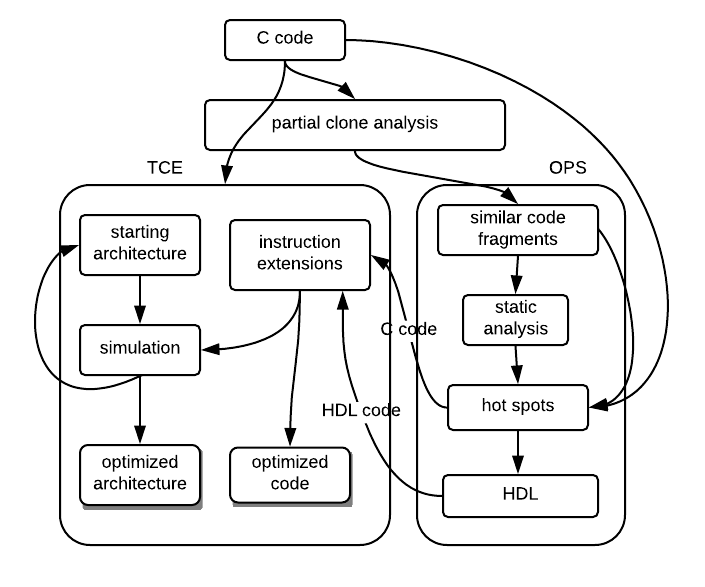
\includegraphics[height=8cm]{img/CodesignFlow.png}
\end{frame}

\begin{frame}{Что делать с клонами}
\framesubtitle{как их быстро искать}
  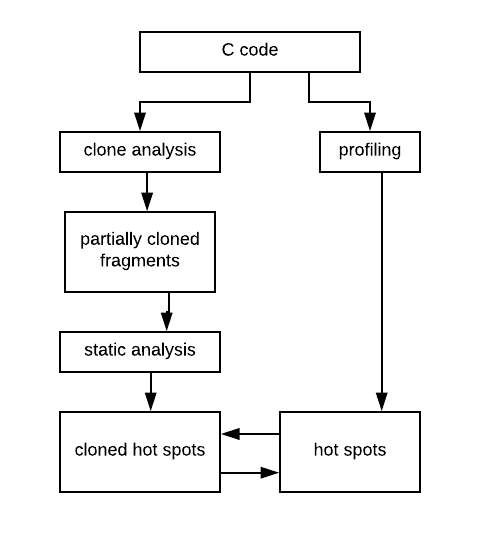
\includegraphics[height=8cm]{img/ClonesFlow.png}
\end{frame}

\begin{frame}{Примеры}
  \framesubtitle{CHStone}
  \begin{table}[htp]
	\begin{centering}
\begin{tabular}{ l c c c c }
\hline
имя программы & всего строк & число фрагментов & \% похожих строк & похожих строк \\
adpcm.txt &	810 &	15	& 35.93 &	291 \\
aes.txt &	797 &	42 &	61.98 &	494     \\
blowfish.txt &	991 &	6 &	10.49 &	104 \\
dfadd.txt &	491 &	2 &	12.63 &	62   \\
dfdiv.txt &	337 &	0 &	0.00 &	0   \\
dfmul.txt &	314 &	2 &	10 &	31  \\
dfsin.txt & 	665 &	10 &	22.71 &	151 \\
gsm.txt	& 478 &	6 &	13.18 &	63      \\
jpeg.txt &	1529 &	26 &	28.2 &	432 \\
mips.txt &	271 &	4 &	15.13 &	41   \\
motion.txt &	672 &	9 &	 15.18 &	102 \\
\hline
\end{tabular}
\caption{Результаты анализа бенчмарка CHStone}
\label{tab:CHStone}
\end{centering}
\end{table}
\end{frame}

\begin{frame}[fragile]
  \framesubtitle{интересные фрагменты}
  
\noindent
\begin{tabular}{|p{6cm}|p{6cm}|}
Участок 1  &  Участок 2 \\
\begin{lstlisting}
for (j = 0; j < nb; ++j)               
{                                      
statemt[j*4]=ret[j*4];           
statemt[1+j*4]=ret[1+j*4];   
statemt[2+j*4]=ret[2+j*4];   
statemt[3+j*4]=ret[3+j*4];   
}                                      
return 0;                              
}                                      
\end{lstlisting}&
\begin{lstlisting}
for (i = 0; i < nb; ++i)
{
statemt[i*4]=ret[i * 4];
statemt[1+i*4]=ret[1+i*4];
statemt[2+i*4]=ret[2+i*4];
statemt[3+i*4]=ret[3+i*4];
}
return 0;
}
\end{lstlisting}
\end{tabular} 
\label{clone_listing_ex}
  
\end{frame}

\begin{frame}[fragile]
\framesubtitle{интересные фрагменты}
\begin{lstlisting}[frame=single]
	x = (statement[(i + 1) % 4 + j * 4] << 1);
	if ((x >> 8) == 1)
	  x ^= 283;
	x = (x << 1);
	if ((x >> 8) == 1)
	  x ^= 283;
	x ^= statement[(i + 1) % 4 + j * 4];
	x = (x << 1);
	if ((x >> 8) == 1)
\end{lstlisting}
\label{clone_listing}
\end{frame}

\begin{frame}{Перспективы}
  %\framesubtitle{Перспективы}
  
\end{frame}


\begin{frame}[allowframebreaks]
        \frametitle{References}
        \bibliographystyle{amsalpha}
        \bibliography{references.bib}
\end{frame}

\end{document}